\documentclass[letterpaper, 12pt]{article}
\usepackage[american]{babel}
\usepackage[utf8]{inputenc}
\usepackage[citestyle=apa,style=apa,backend=biber]{biblatex}
\usepackage[margin=1in]{geometry}
\usepackage{graphicx}
\usepackage{caption}
\usepackage{float}
\usepackage{array}
\setlength\bibitemsep{2\itemsep}
\DeclareLanguageMapping{american}{american-apa}
\addbibresource{bibliography.bib}

% my version of latex does not support this character apparently..
\DeclareUnicodeCharacter{2212}{-}

\begin{document}
\begin{titlepage}
\centering
	\vspace*{5.75cm}
	{\huge\bfseries Final Report\par}
	{\large Parallelizing Machine Learning to Optimize Parameters in Genetic Algorithms\par}
	\vspace{2cm}
	Blair Urish\\
	Dan Wagner\\
	Kansas State University\\
	College of Engineering\\
	Department of Computer Science\\
	\vspace{1cm}
	Dr. Bin Liu\\
	Professor\\
	Department of Chemical Engineering\\
	\vspace{1cm}
	December 15, 2017
\end{titlepage}

\begin{abstract}
\thispagestyle{plain}
\begin{flushleft}
	It is difficult for traditional materials to have some desirable traits that often conflict with one another.  Hybrid materials are crafted to solve this, but the compounds are difficult to identify.  Using machine learning and genetic algorithms to locate the traits of these compounds has had success but is inefficient in computing power.  Thus, we propose an approach to parallelize the process by distributing the work across several nodes in a master-slave relationship.  This method will allow the computation time to be spread across chunks of data, and result in an overall lower run time.
\end{flushleft}
\end{abstract}

\begin{flushleft}

\section*{Background Research}
Many fields require materials with properties that often conflict or trade off with one another. (\cite{Narayanan}; \cite{Ritchie}).  Examples of such properties are low density, high strength, and high flexibility.  In most cases, it is difficult or impossible for traditional materials to exhibit combinations of these properties. Therefore, it is necessary to use hybrid materials that have organic and synthetic components. However, it is difficult to identify these compounds. (\cite{Narayanan}; \cite{Wight}).\\
~\newline
Narayanan et. al. discuss two methods of identifying the components needed to create a hybrid material. The first
method discussed is known as the Reactive Force Field (ReaxFF). The authors state that ReaxFF can describe ``bond formation/dissociation, chemical reaction pathways, and transition states in a diverse class of materials.'' However, they note a major issue with ReaxFF: efficiency. ReaxFF requires a large amount of computing power to do its calculations. Many scientists require running simulations with large sample sizes to which ReaxFF does not scale. \\
~\newline
Bond order potentials (BOP) are a different approach that Narayanan et. al. believe could be significantly more
efficient than ReaxFF. They present an approach that combines Tersoff-Brenner modeling with machine learning that
allows for approximations of the attributes needed to describe the hybrid materials mentioned earlier. The goal
with this technique is to provide fairly accurate results compared with ReaxFF. The authors note that
ReaxFF will still be required for certain heterostructures like oxides. \\
~\newline
However, as noted by Dr. Bin Liu, this machine learning algorithm alone is still not performing as well as 
certain scientists require. He believes that it is possible to introduce parallelization to this existing
algorithm in order to further improve performance. In the next section, we will discuss the approach that we
will be taking in order to parallelize this algorithm.  Following that, we will present our conclusions and future work preparations.

\newpage
\section*{Methodology}
 The overall design process can be seen in the following figure.

 \begin{figure}[H]
 	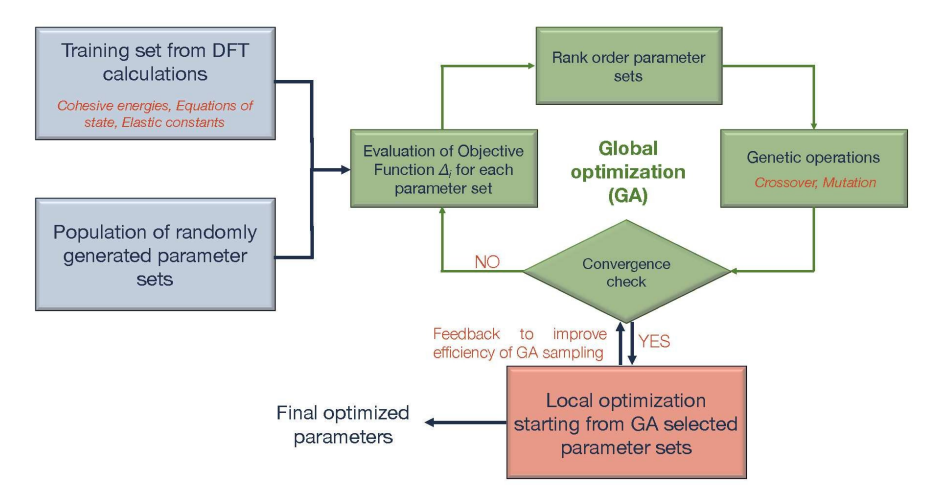
\includegraphics[width=\linewidth,height=10cm,keepaspectratio]{flowchart.png}
 	\caption[Overall Flow of Genetic Algorithm Process]{Overall Flow of Genetic Algorithm Process. Adapted from \cite{Narayanan}}
 	\label{fig:arch}
 \end{figure}

We will begin by discussing the hardware used for our project, then we will discuss the generation of parameter sets and the evaluation of the objective function for each individual first, as these
two processes work closely together. To conclude the section, we will discuss the genetic algorithm and the simplex method. 

\subsection*{Hardware}

We will realize this solution using several nodes on the Beocat supercomputing cluster.  Initially, we plan to restrict our usage to the Elf class nodes for benchmarking. Their specifications can be seen in the accompanying table.
~\newline

\begin{table}[ht]
	\centering
	\caption{Beocat Elf Node Specifications}
	\label{nodespecs}
	\begin{tabular}{|l|l|}
		\hline
		Processors           & 2x 8-Core Xeon E5-2690               \\ \hline
		RAM                  & 64GB                                 \\ \hline
		Hard Drives          & 1x 250GB 7200 RPM SATA               \\ \hline
		NICs                 & 4x Intel I350                        \\ \hline
		10GbE/QDR Infiniband & Mellanox Technologies MT27500 Family \\ \hline
	\end{tabular}
\end{table}

\subsection*{Individual Generation and Fitness Evaluation using LAMMPS}

Before the genetic algorithm can begin, we needed to generate random parameter sets which will function as individuals for the genetic algorithm. 
A parameter set consists of 11 parameters, each of which represent atomic traits. We were given starting values for these traits and were told to vary them by $\pm$ 25\%. 
With this information, we decided to create a C++ class to represent an individual and help keep our data organized. This class holds the parameter values in a map, which maps the parameter name to its value. 
This was chosen because it makes iterating through the parameter set extremely easy, since C++ maps support foreach loops by default. When the class is constructed, we use the new
random number generator in C++ 11 to generate values for each trait in the parameter map. Once constructed, users of the class can easily access the parameter map using the class's 
indexer, which we have overrided to index directly into the map. \\
~\newline
Our Individual class also hold another very important value for our algorithm: the fitness. This value is calculated at the time of class construction. In order to get this value,
we have to use LAMMPS. This proved to be one of the most challenging parts of this program. LAMMPS is not a very easy program to use and much of the data that we originally received
from Dr. Liu did not work correctly and we did not know how to use it. We first tried to run LAMMPS as a standalone program from the terminal, just to get an idea of what kind of
input it expects and what kind of output it gives. 

\subsection*{Genetic Algorithm}

~\newline
One computing node will be designated as the master node, while several other nodes will be the slave nodes.  OpenMPI in C++ will be used in order to facilitate communication between the master and slaves. The master node will receive a population of randomly generated parameter sets and the training set provided.  It will partition the population into subsets and send the sets to slave nodes for evaluation.  The size of these partitions could vary; ideally, each node would contain a chunk that fits wholly within the L3 cache. Each slave node will evaluate the fitness of each individual within their subset. Then, they will transfer the results back to the  master node for modification via trait crossover and mutation. The best one hundred individuals will be retained for subsequent generations.\\

~\newline
Our Genetics class will handle the crossover of traits and the mutation of $\pm$ 33\% of the individuals.  Crossovers take two individuals and swaps their traits starting at a random trait number.  Then, the appropriate trait is found and the individuals exchange their values for that trait.  At the end of the crossover, the two individuals' fitnesses need to be recalculated and are done so with a call to LAMMPS.  Mutations are performed on a single individual that is randomly chosen from the dataset.  The appropriate trait is found (similarly to crossovers) and its value in the individual is recalculated.  Afterwards, its fitness is reevaluated.

~\newline
~\newline 
This process will continue until the genetic algorithm fails to return better individuals than the previous run.  At this convergence step, the twenty best individuals will be selected to undergo local minimization by the Simplex method.  Finally, the most optimized individual results will be the best set of parameters for this generation. \\
~\newline
The Large-scale Atomic/Molecular Massively Parallel Simulator (LAMMPS) package will be used to evaluate individuals' fitness.  This software is a classical molecular dynamics code developed by Sandia National Laboratories.  It has optimized integrations with OpenMPI, which will fit into our overall design very well. \\
~\newline 
A base run time of one hour per population has been established by Dr. Bin Liu.  Our implementation will run the same dataset, with the results and run times being compared for accuracy and performance.  We are expecting at least a factor of ten speedup on a single core by using OpenMPI and distributing the work across several nodes.


\section*{Simplex Method}
The Simplex Method is a way of locally minimizing parameters of an equation.  Each parameter is constrained to a certain range and permuted slightly in an attempt to minimize a functional value.  Typically, the equations are set up in matrix form.  On each iteration, the simplex advances towards a local minimum. 

\newpage
\section*{Conclusion}
We have proposed a way to parallelize the process of optimizing hybrid material properties in genetic algorithms.  A global single-population master-slave approach will divide up the population into subsets of individuals and then pass them to slave nodes.  Slaves will operate on their data with LAMMPS and evaluate the fitness of each individual.  These results will be sent back to the master node who will perform genetic operations on them.  We expect a factor of ten speedup, at the minimum, to be exhibited on a single core as we work.

\section*{Future Work}
Future work will include implementing the master-slave genetic algorithm using OpenMPI and C++ with an interface into LAMMPS.  The software will be benchmarked and checked for accuracy.
\newpage
\printbibliography

\end{flushleft}
\end{document}
